\documentclass[11pt,a4paper,oneside]{article}


\usepackage[T2A]{fontenc}
\usepackage[utf8]{inputenc}
\usepackage[english,russian]{babel}
\usepackage[russian]{olymp}
\usepackage{graphics}
\usepackage{wrapfig}
\usepackage{amsmath}
\usepackage{amssymb}
\usepackage{epigraph}
\usepackage{graphicx}


\newcommand{\qo}{\textquotesingle}
\newcommand{\qq}{\textquotesingle~}

\contest{ACM ICPC Kyrgyzstan Subregional 2015}{Бишкек}{1 ноября 2015 года}    

\binoppenalty=10000
\relpenalty=10000
\exhyphenpenalty=10000

\renewcommand{\t}{\texttt}

\createsection{\Note}{Примечание}

\renewcommand{\defaultmemorylimit}{256 мегабайт}

\begin{document}

\begin{problem}{Задача F. Краска}{1 секунда}{32 мегабайта}

На плоскости лежит единичный квадрат, стороны которого параллельны осям координат, намазанный краской. Возможны команды сдвига на единицу длины:
R (сдвиг вправо), L (сдвиг влево), U (сдвиг вверх), D (сдвиг вниз).
После буквы записывается натуральное число, меньшее 10, означающее количество повторений данной команды.
Найти площадь окрашенной части плоскости после выполнения четырех таких команд с повторениями.


\InputFile
Одна строка, в которой записаны четыре команды - первый знак – одна из букв R, L, U, D,  второй знак – одна из цифр 1..9, разделенные одинарными пробелами.


\OutputFile
Одно натуральное число.


\Examples

\begin{example}%
\exmp{
L5 R8 U2 U1
}{
12
}%
\exmp{
D4 R1 U4 L1
}{
10
}%
\end{example}

\vspace{0.3cm}
\medskip\noindent
\textbf{Пояснение к примерам.}


Части плоскости, окрашенные после выполнения команд в первом и втором примерах показаны на рисунках 1 и 2 соответственно.

\begin{figure}[ht]
\centering
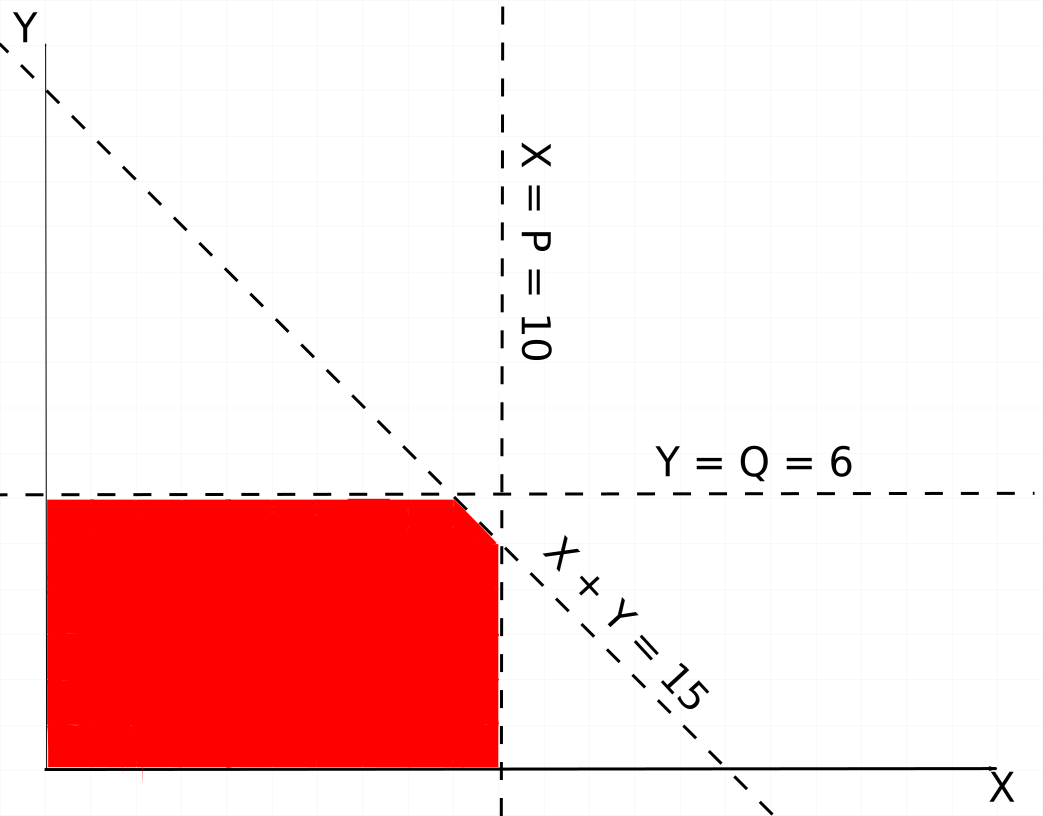
\includegraphics[width=0.4\textwidth]{drawing.pdf}
\caption{Окрашенная часть плоскости в примере 1.}
\end{figure}


\begin{figure}[ht]
\centering
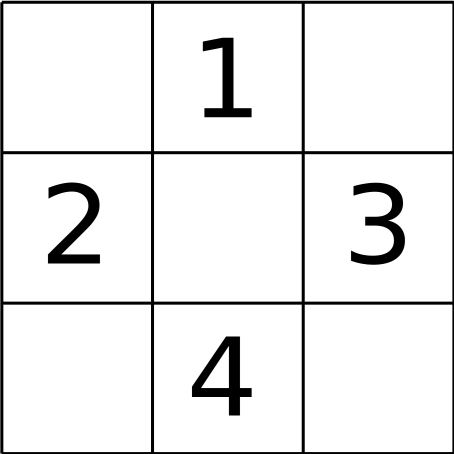
\includegraphics[width=0.145\textwidth]{drawing2.pdf}
\caption{Окрашенная часть плоскости в примере 2.}
\end{figure}


\vspace{1.0cm}
\hfill \textit{Автор задачи: Панков П.C.}
\medskip\noindent




\end{problem}


\end{document}
%%% Local Variables:
%%% mode: latex
%%% TeX-master: t
%%% End:
